\documentclass[a4paper, 12pt]{article}

\usepackage{amsmath}
\usepackage[utf8]{inputenc}
\usepackage{graphicx}
\usepackage{caption}
\usepackage{physics}
\usepackage{tikz}
\usepackage{tkz-graph}
\usepackage{tikzscale}
\usetikzlibrary{arrows}
\usepackage{parskip}

\captionsetup{width=0.8 \linewidth}

\begin{document}

\title{\vspace{-6em}\textbf{Homework 3}\\ \Large Information Theory for Complex Systems \vspace{-1em}}
\author{}
\date{\vspace{-3.2em}}

\pagenumbering{gobble}

\maketitle

\textbf{a)} The given initial state can produce all permutations of symbols except for 010. The remaining 7 patterns ran through rule 174 can be paired as follows:
\begin{table}[ht!]
    \centering
    \begin{tabular}{|c|c|c|c|}
        $110 \rightarrow 0$ & $100 \rightarrow 0$ & $000 \rightarrow 0$ & \\
        $111 \rightarrow 1$ & $101 \rightarrow 1$ & $001 \rightarrow 1$ & $011 \rightarrow 1$
    \end{tabular}
\end{table}
Each column contains the same patterns, but with the last bit flipped (which results in a flipped output). This is exactly what is described by equation (4.5) from the course book. Therefore rule 174 with this FSA giving the initial state is almost reversible. By attempting all possible combinations I also ruled out 010 being produced in a future time steps, which could've destroyed the almost reversability..

\textbf{b)} With an optimal encoding the FSA can be equivalently described by
\vspace{-1.5em}
\begin{figure}[ht]
\begin{center}
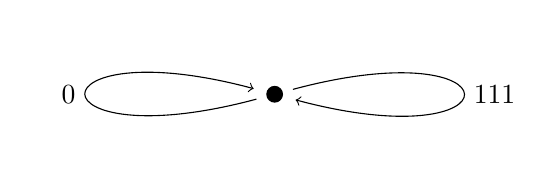
\begin{tikzpicture}[main node/.style={circle,draw,fill,inner sep=2pt,outer sep=4pt},scale=6]
    \node[main node] (1) {};
    \path
        (1) edge [loop left] node {0} (1)
            edge [loop right] node {111} (1);
\end{tikzpicture}
\end{center}
\end{figure}

\vspace{-1.5em}
This FSA trivially has the entropy per symbol $s_{opt} = 1$. In the limit where the sequence of symbol goes to infinity, the original FSA produces twice as many symbols as this optimal FSA. Therefore the entropy per symbol (entropy density) at $t = 0$ is $s = 1/2$.

\textbf{c)}  Group the symbols into pairs, highlight which pattern in rule 174 is applied at the  edges and replace the rule applications with their results.
\begin{figure}[ht!]
    \centering
    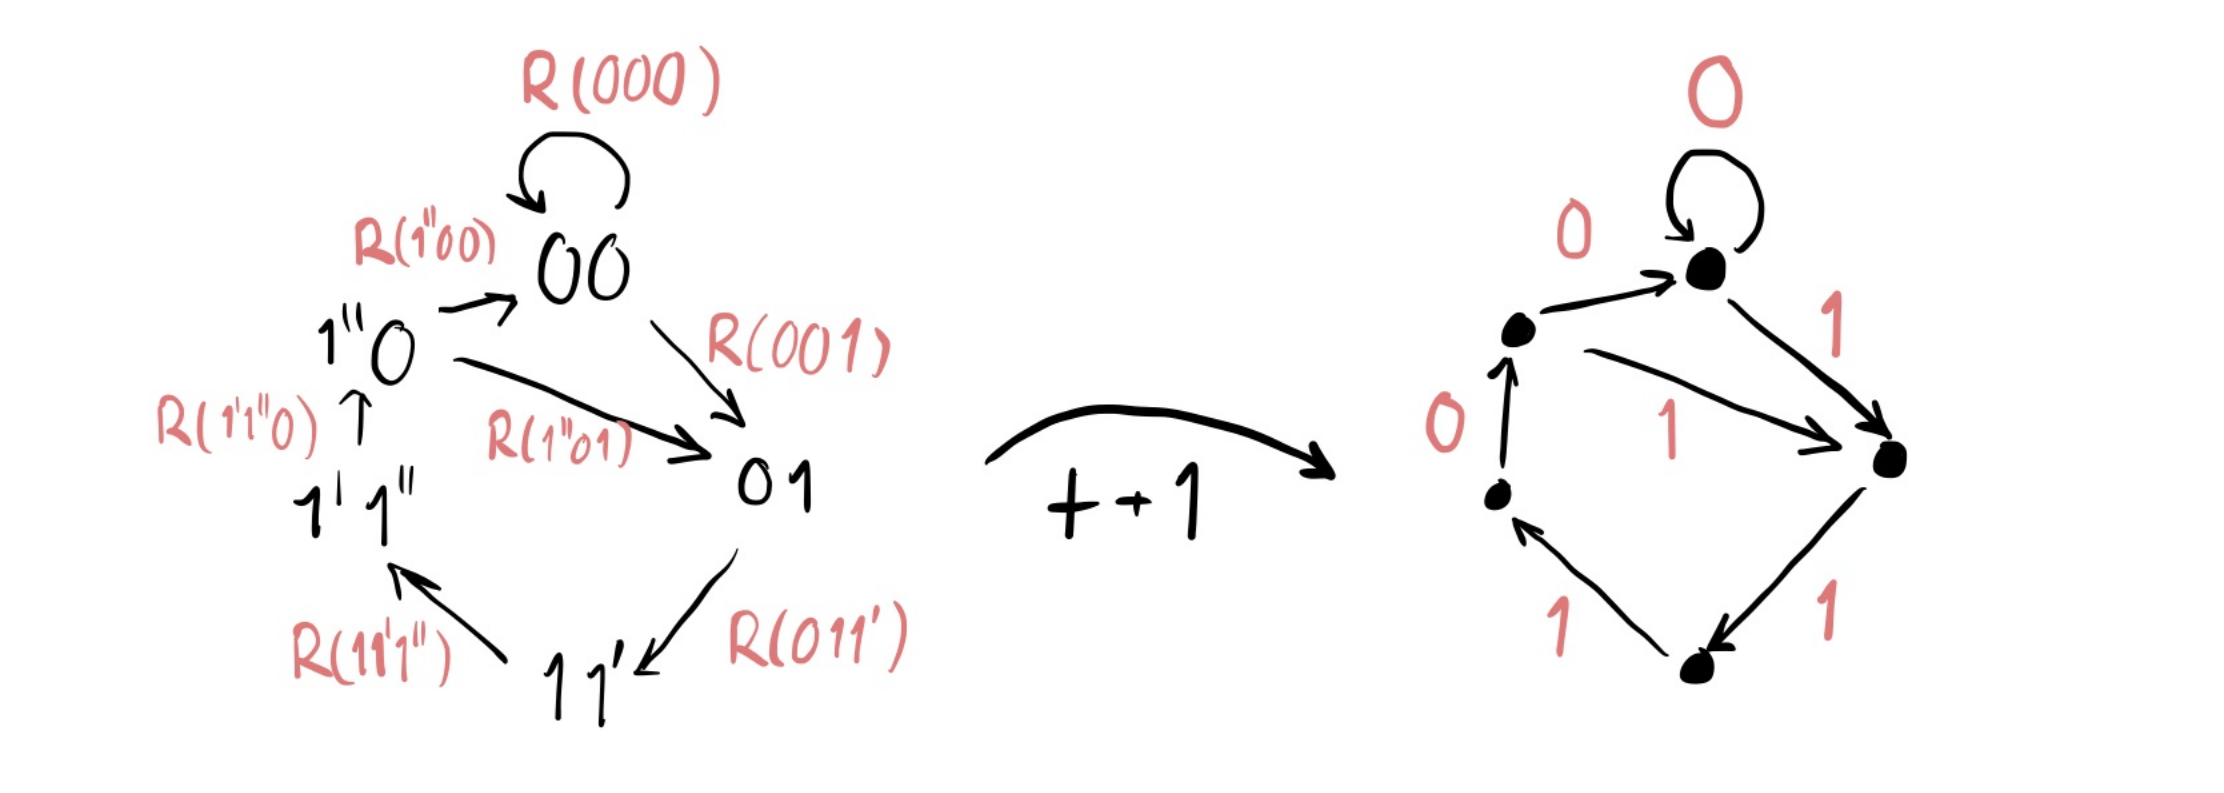
\includegraphics[width=0.5 \linewidth]{Info Theory-12.png}
\end{figure}

\textbf{d \& e)}
The FSA at $t = 1$ can also be reduced to the same FSA as before, with the same probabilities. Therefore the entropy calculation is the same (the first equivalence doesn't reduce the amount of symbols produced) giving $s(t=1) = 1/2$. Moving to $t=2$ from this point is applying the same process again, with identical starting conditions and results, giving $s(t=2) = 1/2$.
\begin{figure}[ht!]
    \centering
    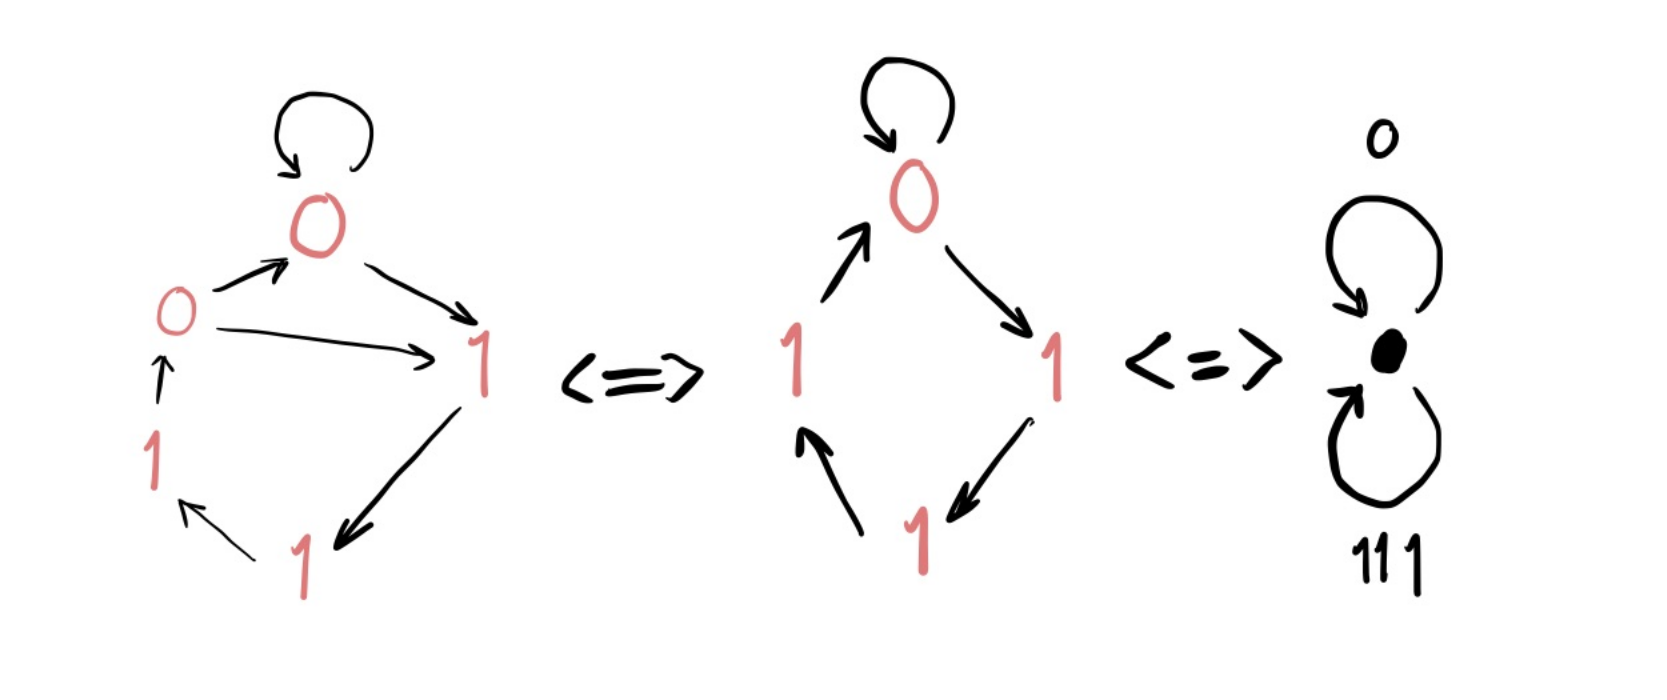
\includegraphics[width=0.5 \linewidth]{d.png}
\end{figure}

\end{document}
